A metodologia adotada nesta pesquisa se envolve a modelagem do conjunto de dados \textit{``Loan Data for Dummy"},
retirado da plataforma \textit{Kaggle},
visando a compreensão e modelagem de padrões associados a operações de empréstimos. Dois métodos distintos, 
Regressão Logística e Redes Neurais, serão empregados para investigar as relações existentes nos dados e aprimorar as previsões.
A implementação desses modelos será realizada utilizando tanto a linguagem de programação R quanto Python.
Além disso, a técnica SHAP (\textit{Shapley Additive Explanations}) será integrada para proporcionar
uma interpretação aprofundada do modelo de redes neurais, ampliando a transparência nas decisões preditivas. 



\subsection{Conjunto de dados}

O banco de dados \textit{``Loan Data for Dummy"} é uma base de dados do Kaggle, projetada para simular informações relacionadas 
a operações de empréstimos. Desenvolvido para fins educacionais e de pesquisa, esse conjunto tem sua origem de um modelo de 
banco \textit{``peer to peer"} sediado na Irlanda, no qual o banco disponibiliza recursos a potenciais clientes, 
obtendo lucros com base no risco que assume. 
Os dados disponíveis no Kaggle representam uma versão fictícia de uma situação real, com a maior parte dos dados manipulados
ou criados sinteticamente para preservar as informações dos clientes originais.

A variável resposta que desejamos modelar é a ``Condição do empréstimo". Através dessa variável, é 
possível discernir se um empréstimo foi classificado como ``bom" ou ``ruim", proporcionando uma avaliação da qualidade e 
risco associados a cada transação. No contexto deste conjunto de dados, a ``Condição do empréstimo" é uma variável binária,
onde ``0" indica um empréstimo em boas condições e ``1" indica o contrário.

\subsubsection{Variáveis}

A base de dados é composta por 30 variáveis, incluindo a variável resposta, e existem 887379 observações.
A fim de estudar ``Condição do empréstimo" foram utilizadas algumas variáveis presentes na base de dados, como:

\begin{enumerate}
  \item \textbf{Tempo de emprego}: Representa o tempo (em anos) de emprego do solicitante expresso numericamente. 
  \item \textbf{Tipo de residência}: Indica o status de moradia do solicitante(por exemplo: proprietário, inquilino ou outra forma de ocupação residencial). 
  \item \textbf{Renda anual}: Indica a renda anual do solicitante, uma medida crucial para avaliar a capacidade de pagamento do empréstimo. 
  \item \textbf{Valor do empréstimo}: Representa o valor do empréstimo solicitado pelo requerente.
  \item \textbf{Prazo}: Indica o prazo do empréstimo, especificando o período de tempo durante o qual o empréstimo deve ser reembolsado (por exemplo: 36 meses).
  \item \textbf{Tipo de aplicação}: Refere-se ao tipo de aplicação, indicando se é uma aplicação individual ou conjunta.
  \item \textbf{Finalidade}: Descreve a finalidade do empréstimo(por exemplo: como consolidação de dívidas, compra de casa, educação, entre outros).
  \item \textbf{Tipo do juros}: Indica a natureza dos pagamentos de juros(por exemplo: se são fixos ou variáveis). 
  \item \textbf{Taxa de juros}: Representa a taxa de juros associada ao empréstimo.
  \item \textbf{Grau}: Refere-se à classificação de risco do tomador de empréstimo atribuída pela instituição financeira (por exemplo: A, B, C, etc).
  \item \textbf{DTI}: Significa ``Debt-to-Income" (Dívida-para-Renda) e representa a proporção entre as dívidas mensais e a renda mensal do requerente, proporcionando uma medida da capacidade de pagamento.
  \item \textbf{Valor bruto pago}: Representa o valor total pago, incluindo o principal e os juros, ao final do empréstimo.
  \item \textbf{Valor líquido pago}: Indica o total de principal (quantia inicial do empréstimo) recuperado até o momento.
  \item \textbf{Valor recuperado}: Representa o valor recuperado em caso de inadimplência ou perda.
  \item \textbf{Parcelas}: Indica o valor da parcela mensal que o requerente do empréstimo deve pagar, incluindo tanto o principal quanto os juros.
  \item \textbf{Região}: Indica a região geográfica associada ao requerente do empréstimo.
\end{enumerate}



\subsubsection{Limpeza dos dados}

Para diminuir a complexidade da base de dados, as variáveis passaram por 3 critérios de avaliação antes de serem utilizadas
nos modelos:

\begin{enumerate}
  \item Remoção de variáveis irrelevantes para o estudo;
  \item Exclusão de variáveis que geram a mesma informação;
  \item Extração de variáveis presentes em apenas uma das categorias da variável resposta.
\end{enumerate}

No item 1. destaca-se a variável ``ID" como independente da variável resposta, 
atuando unicamente como identificador do cliente, sem exercer influência no resultado final do modelo.

O item 2. se refere à situação da base de dados em que o autor realizou uma rotulação numérica de variáveis 
já categorizadas, como por exemplo: 
``Tipo de juros" e ``Tipo de juros Cat", onde na primeira variável tem as opções ``Juros simples" e ``Juro compostos" e na segunda variável
o autor associa os números ``1" e ``2", respectivamente, a essas variáveis.

O item 3. exclui variáveis que desempenham funções em apenas uma das categorias da variável resposta. Como é o caso da 
variável ``Recuperações totais", visto que esta mesma é presente apenas no caso do cliente ter sido inadimplente, se relacionando
com a categoria ``Empréstimo ruim" da variável resposta. Para o caso de ``Empréstimo bom" os valores da variável são sempre zero.

Com isso a base de dados ficou da seguinte maneira:

\begin{table}[h]
  \centering
  \begin{tabular}{l|c}
  \hline
  \textbf{Base de dados} & \textbf{Número de Colunas} \\ \hline
  Antes da limpeza & 30 \\ 
  Depois da limpeza & 18 \\ \hline
  \end{tabular}
  \caption{Número de colunas antes e depois da preparação dos dados}
  \label{table:columns_before_after}
\end{table}

Com o tratamento dos dados realizado, foi feita a separação dos dados para a modelagem dos dois modelos.


\begin{table}[h]
  \centering
  \begin{tabular}{l|c}
  \hline
  \textbf{Tipo de dado} & \textbf{\% dos dados originais} \\ \hline
  Treino & 70\% \\ 
  Validação & 10\% \\
  Teste & 20\% \\ \hline
  \end{tabular}
  \caption{Divisão dos dados para a modelagem dos modelos de regressão logística e redes neurais}
  \label{table:divisao_dados}
\end{table}



\subsection{Modelagem dos dados}

\subsubsection{Regressão logística}

\begin{figure}[H]
  \centering
  \caption{Fluxograma da implementação do modelo logístico}
  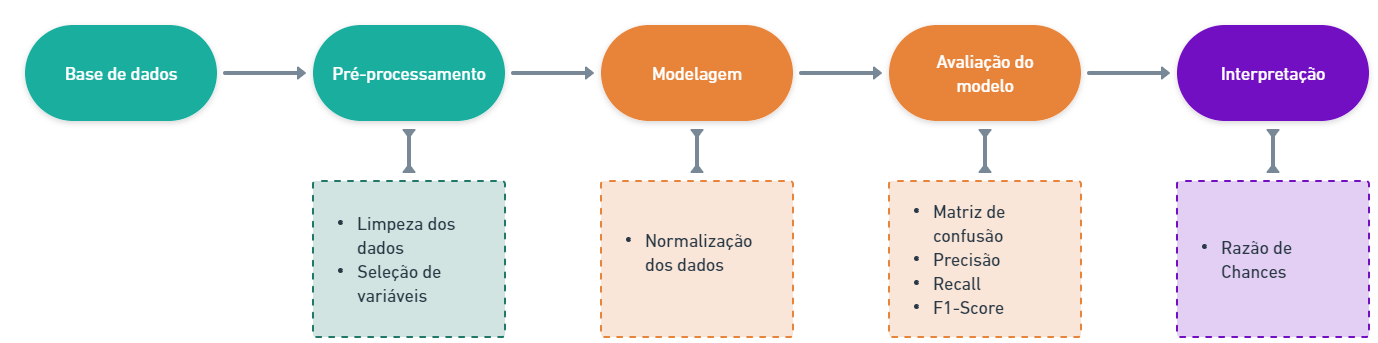
\includegraphics[width=1\textwidth]{imagens/flugrama_logistico.png}
  \subcaption*{Fonte: Autoria própria}
  \label{fig:imagens/flugrama_logistico.png}
\end{figure}

A metodologia para a implementação da regressão logística incluiu várias etapas essenciais para 
garantir a robustez e eficácia do modelo. Inicialmente, foi realizada uma cuidadosa etapa de pré-processamento, 
que envolveu a limpeza e tratamento das variáveis. Durante essa fase, foram identificados e tratados 
possíveis valores ausentes, outliers e erros nos dados, contribuindo para a qualidade do conjunto de dados.

Outro aspecto crítico foi a categorização adequada das variáveis, quando aplicável. Isso incluiu a transformação
de variáveis categóricas em formatos adequados para análise estatística, garantindo que todas as variáveis 
estivessem em uma forma consistente para o modelo de regressão logística.

Para facilitar a interpretação do modelo, os valores das variáveis
 normalizados, usando uma padronização que retorna dados em uma escala com média zero e
desvio padrão unitário.

Dada a natureza desbalanceada do conjunto de dados, onde as classes ``Empréstimo bom" e ``Empréstimo ruim" têm
proporções significativamente diferentes, foi aplicado um corte diferente de 0.5 no momento de dividir as predições
do modelo. Foi utilizada a proporção da categoria minoritária em relação à classe majoritária como ponto de corte
\cite{agresti2002}.

Tendo o modelo definido, foi feita uma avaliação das predições do modelo no conjunto de teste, usando métricas
apropriadas para problemas de classificação, como precisão, recall, F1-score e matriz de confusão. 
Essas métricas permitiram uma compreensão abrangente do desempenho do modelo, especialmente no que diz respeito à
capacidade de prever corretamente os casos de ``Empréstimo ruim" e ``Empréstimo bom".


\subsubsection{Rede neural}

\begin{figure}[H]
  \caption{Fluxograma da implementação da rede neural}
  \centering
  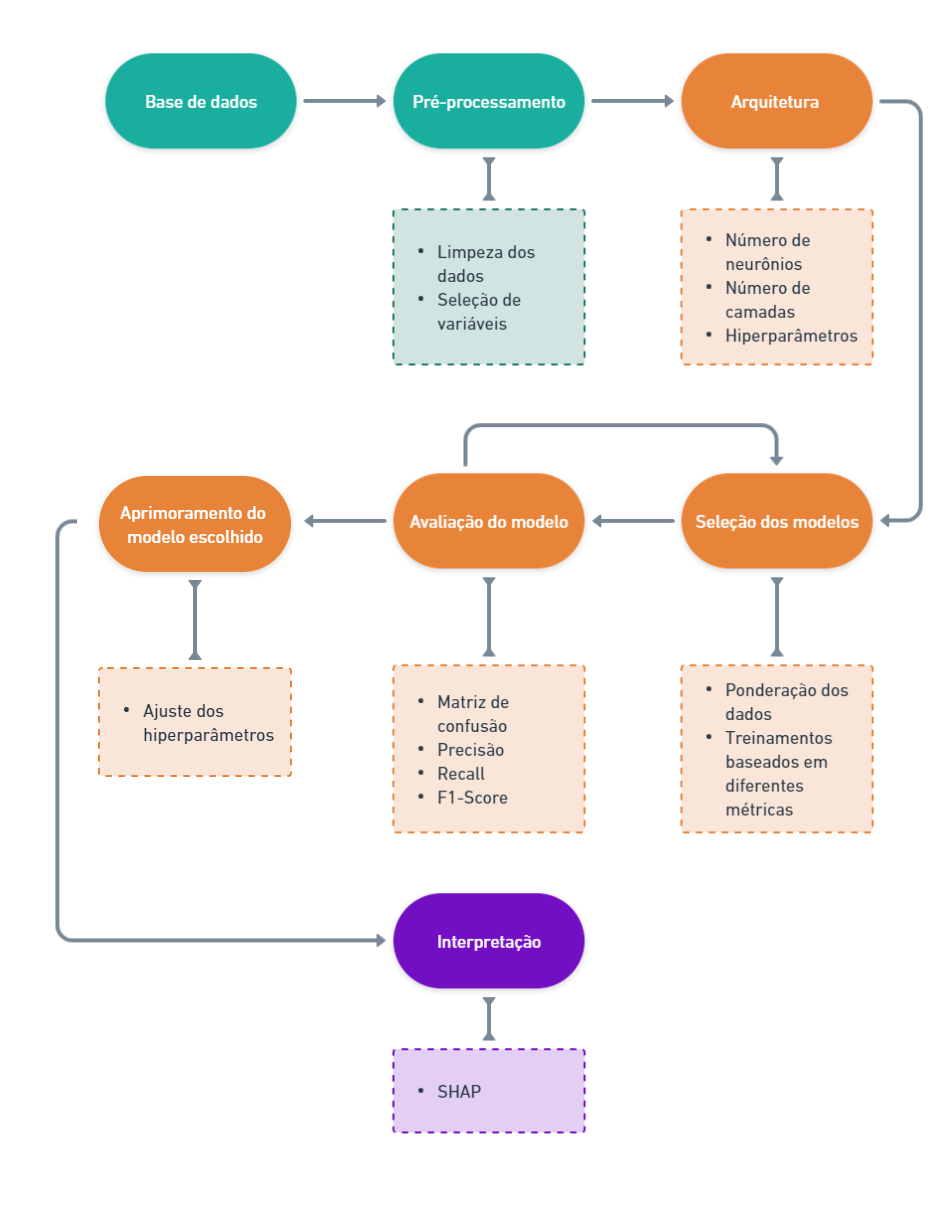
\includegraphics[width=0.7\textwidth]{imagens/flugrama_rede_neural.png}
  \subcaption*{Fonte: Autoria própria}
  \label{fig:imagens/flugrama_rede_neural.png}
\end{figure}



A  construção e ajuste das redes neurais envolveu diversas etapas cruciais 
para garantir a eficácia do modelo. Inicialmente, foi realizada uma fase de pré-processamento, que consistiu
na limpeza e tratamento das variáveis. Durante esse estágio, foram tratados valores ausentes, outliers e possíveis
erros nos dados, contribuindo para a qualidade do conjunto de dados. Essa etapa foi a mesma apresentada pelo
modelo logístico.

A escolha da arquitetura inicial foi um passo importante. Foi necessário definir o número de camadas ocultas,
a quantidade de neurônios em cada camada e a função de ativação a ser utilizada. Essas escolhas iniciais foram 
baseadas tanto em conhecimentos prévios do problema quanto em experimentações para encontrar a configuração que 
melhor se adequava aos dados. 
E para isso foi utilizado uma rede neural baseada na Figura \ref{fig:imagens/arc_rede_neural.png}:

\begin{figure}[H]
  \centering
  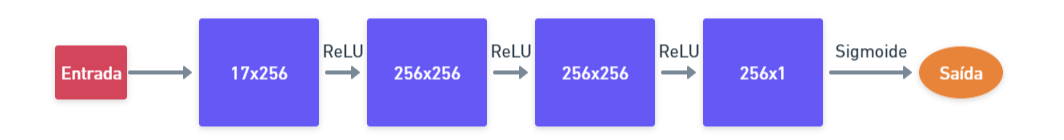
\includegraphics[width=1\textwidth]{imagens/arc_rede_neural.png}
  \caption{Arquitetura de rede neural inicial}
  \label{fig:imagens/arc_rede_neural.png}
\end{figure}


Diversos modelos de redes neurais foram desenvolvidos e treinados em contextos variados,
 considerando abordagens distintas, tais como:

\begin{itemize}
  \item Tratamento para dados desbalanceados;
  \item Ajuste dos modelos otimizando métricas de treinamento variadas;
  \item Ponderação das classes da variável resposta.
\end{itemize}

\begin{figure}[H]
  \caption{Fluxograma da escolha dos modelos de redes neurais estimados}
  \centering
  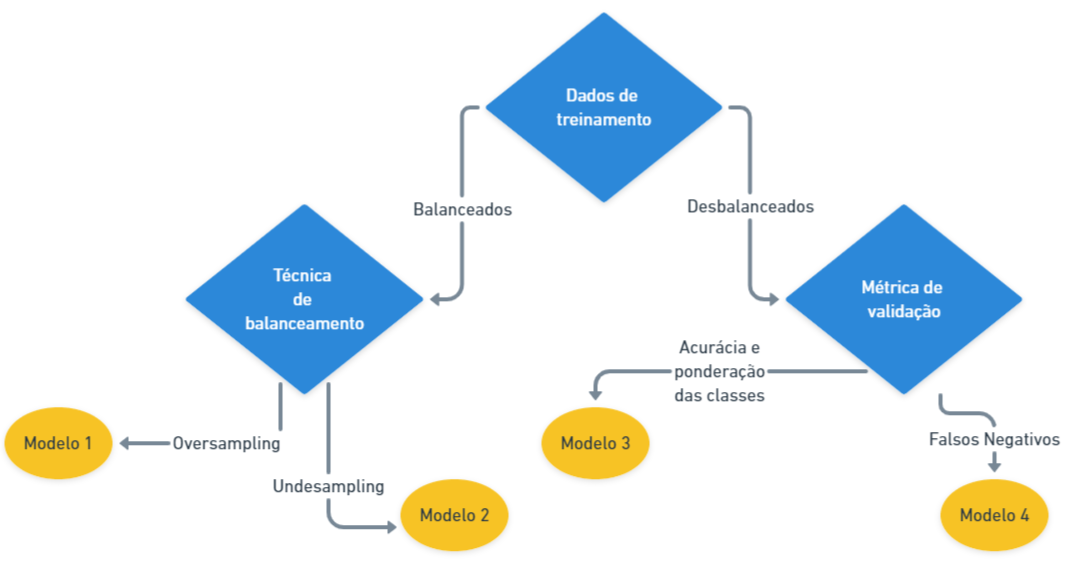
\includegraphics[width=0.9\textwidth]{imagens/fluxograma_selecao_modelo_neural.png}
  \subcaption*{Fonte: Autoria própria}
  \label{fig:imagens/fluxograma_selecao_modelo_neural.png}
\end{figure}



Conforme ilustrado na Figura \ref{fig:imagens/fluxograma_selecao_modelo_neural.png}, o treinamento dos modelos com dados equilibrados, foram empregados dois processos distintos: 
\textit{upsampling} e \textit{oversampling}. No âmbito da modelagem, em que se priorizaram métricas específicas
de treinamento, além da acurácia, métrica padrão, foram considerados o Recall 
e o número de Falsos Negativos. Este último é particularmente crucial em cenários de empréstimos, sendo considerado
o erro mais relevante. Por fim, foi utilizado também um modelo com ponderação nas classes, buscando assim equilibrar 
a classe majoritária. Essas abordagens visaram explorar diferentes aspectos do treinamento para encontrar a 
configuração mais eficaz, adaptada às situações do problema em análise.

Cada modelo foi treinado utilizando 
o conjunto de treinamento e validado para avaliar seu desempenho, no conjunto de validação. 
As métrica de desempenho, geralmente relacionadas
à precisão, recall e F1-score, foi usada para comparar e selecionar os melhores modelos.

O modelo mais promissor foi então submetido a uma etapa de ajuste de hiperparâmetros. Ajustes finos nos 
hiperparâmetros, como taxa de aprendizado, número de épocas de treinamento e tamanho do lote, 
foram realizados para otimizar o desempenho do modelo, utilizando o conjunto de validação.
A arquitetura final do modelo está ilustrada na Figura \ref{fig:imagens/arquitetura_redeneural_vencedor.png}.


\begin{figure}[H]
  \centering
  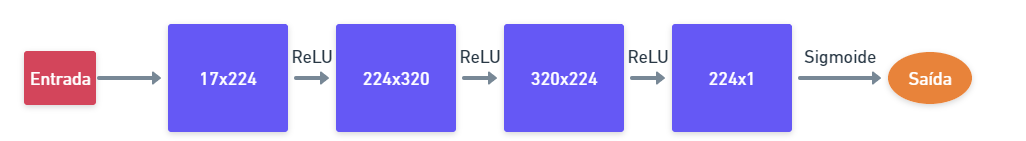
\includegraphics[width=1\textwidth]{imagens/arquitetura_redeneural_vencedor.png}
  \caption{Arquitetura final da rede neural}
  \label{fig:imagens/arquitetura_redeneural_vencedor.png}
\end{figure}

O modelo que apresentou a melhor performance foi utilizando as classes ponderadas e a acurácia como métrica de desempenho.

A avaliação final do modelo ocorreu no conjunto de validação e teste. Essa etapa foi crucial 
para garantir que o modelo não apenas se ajustasse bem aos dados de treinamento, mas também 
generalizasse de maneira eficaz para novos dados. As métricas de desempenho foram novamente
utilizadas para avaliar a capacidade do modelo de fazer previsões precisas e úteis, no conjunto de teste.

\subsection{Interpretação dos modelos}


Definindo os modelos logístico e o de redes neurais, foi feita a interpretação de ambos.
E realizar a interpretações dos modelos é uma etapa crucial na análise de dados, mostrando
 o funcionamento e as relações das variáveis no contexto do problema em questão. 

No caso do modelo logístico, a interpretação se concentrou nos parâmetros estimados para cada variável. 
Esses coeficientes fornecem uma medida da magnitude e direção da influência de cada variável na predição da
 variável resposta. Além disso, a interpretação envolveu a análise da Razão de Chances (RC), que expressa 
 como a chance de o evento ocorrer se torna multiplicativamente maior ou menor com a mudança em uma unidade 
 na variável explicativa.

Para a interpretação da rede neural, utilizou-se a técnica SHAP (\textit{SHapley Additive exPlanations}). 
Essa abordagem proporciona uma compreensão mais profunda ao atribuir a contribuição de cada variável para a saída do 
modelo em nível individual. Com o auxílio de gráficos SHAP, pôde-se observar como cada variável influencia as predições 
e identificar padrões de comportamento em diferentes cenários.


